\documentclass[12pt,a4j]{jarticle}
\usepackage[dvipdfmx]{graphicx}
\usepackage{listings}
\begin{document}
\title{コンピュータリテラシレポート#13}
\author{1920031, 山川竜太郎}
\date{2019/07/19}
\maketitle


\section{課題の再掲}
演習3 ブロックレイアウトの例をそのまま動かしてみなさい。うまく動いたら、grid-template-areaを変更して配置を修たり、サイドバーを右側にしたり、ブロックの数を増減してみなさい。最終的には、自分が自分のサイトを作るときに使いたいと思う色づかいと配置のレイアウトを構成してみなさい。

\section{レポートの本文}

自分がサイトに使いたいと思う配置を構成した。今回は1998年電気通信大学1年生が入学希望の学生に校内を紹介する目的のホームページを作成すると想定した。テキストのサンプルhtmlより変更したのは以下の点である。

\begin{itemize}
  \item デザインを縦4x横4のグリッドデザインに変更した。
  \item 1列目をサイドバーとして使用した。
  \item sectionタグを6つにして、それぞれグリッド1マス分にした。
  \item seciontタグにに対して、borderを引いて隣のseciontとの範囲が分かるようにした。
  \item 2frと1frのグリッドを用意して、まぜて作成した。
\end{itemize}

\subsection{実際に作成したページ}

\begin{center}
  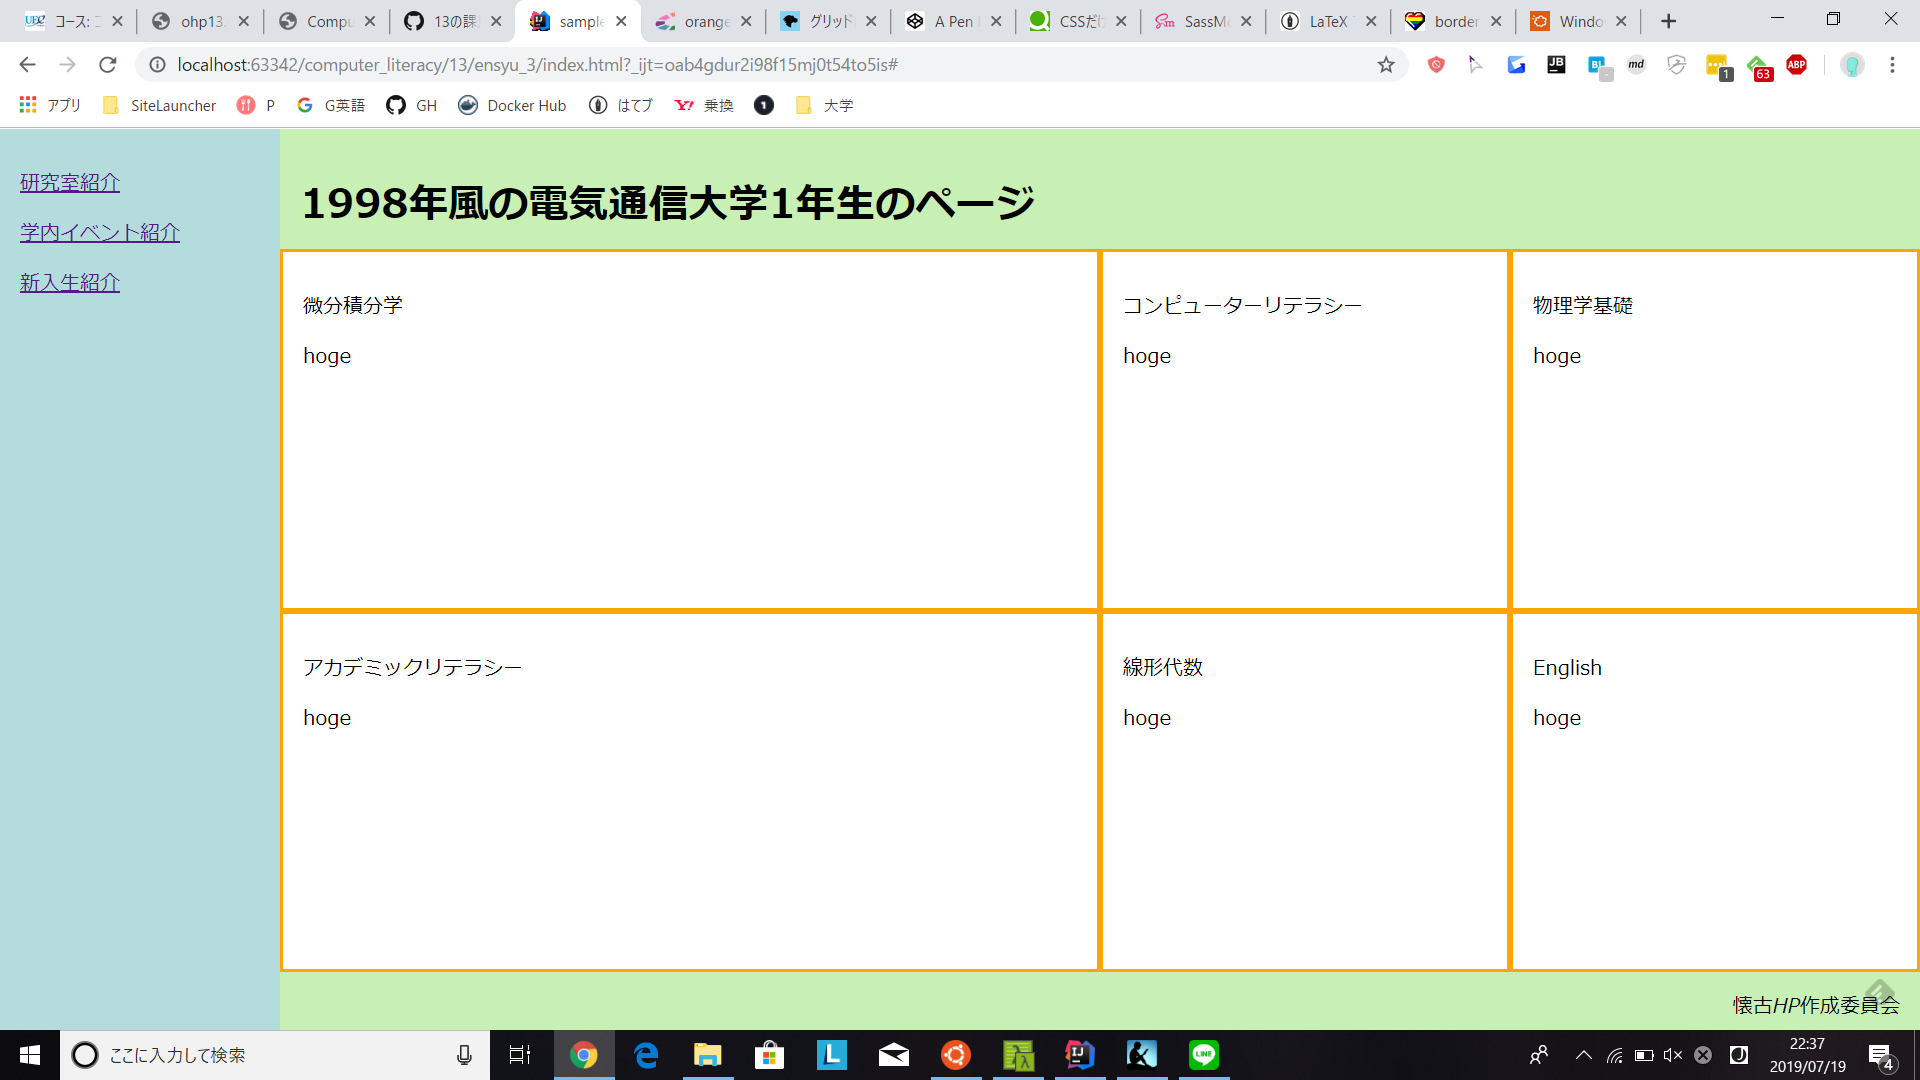
\includegraphics[width=10cm]{./ensyu_3/image.png}
\end{center}

\subsection{ソースコード}

\begin{lstlisting}[basicstyle=\ttfamily\footnotesize, frame=single]

<!DOCTYPE html>
<html>
<head>
    <meta charset="utf-8">
    <title>sample</title>
    <style type="text/css">
        body {
            margin: 0px
        }

        .main {
            display: grid;
            width: 100vw;
            height: 100vh;
            grid-template-areas: "side header header header" "side a b c" "side d e f" "side footer footer footer";
            grid-template-columns: 14em 2fr 1fr 1fr;
            grid-template-rows: 6em 1fr 1fr 3em
        }

        header {
            grid-area: header;
            background: rgb(200, 240, 180);
            padding: 1em
        }

        aside {
            grid-area: side;
            background: rgb(180, 220, 220);
            padding: 1em
        }

        section {
            background: #ffffff;
            padding: 1em;
            border: medium solid #ffa500;
        }

        #a {
            grid-area: a;
        }

        #b {
            grid-area: b;
        }

        #c {
            grid-area: c;
        }

        #d {
            grid-area: d;
        }

        #e {
            grid-area: e;
        }

        #f {
            grid-area: f;
        }

        footer {
            grid-area: footer;
            background: rgb(200, 240, 180);
            padding: 1em
        }

        address {
            text-align: right
        }
    </style>
</head>
<body>
<div class="main">
    <header><h1>1998年風の電気通信大学1年生のページ</h1></header>
    <section id="a">
        <p>微分積分学</p>
        <p>hoge</p>
    </section>
    <section id="b">
        <p>コンピューターリテラシー</p>
        <p>hoge</p>
    </section>
    <section id="c">
        <p>物理学基礎</p>
        <p>hoge</p>
    </section>
    <section id="d">
        <p>アカデミックリテラシー</p>
        <p>hoge</p>
    </section>
    <section id="e">
        <p>線形代数</p>
        <p>hoge</p>
    </section>
    <section id="f">
        <p>English</p>
        <p>hoge</p>
    </section>
    <aside>
        <p><a href="#">研究室紹介</a></p>
        <p><a href="#">学内イベント紹介</a></p>
        <p><a href="#">新入生紹介</a></p>
    </aside>
    <footer>
        <address>懐古HP作成委員会</address>
    </footer>
</div>
</body>
</html>

\end{lstlisting}

\section{考察}

テーマを決めたほうが、デザインに対して意義が生まれる。具体例の一つはサイドバーだが、サンプルではヘッダー部分にはサイドバーがなかったが1998年ごろのサイトは、サイドバーは横1列ごと使用していたデザインが多いのでこのようなデザインにした。2frと1frを混成した場合の挙動が分かっておらず、最初は1行や1列ごとのfr数の上限が決まっていると思った。実際にやってみると、全体の長さに対して、emで長さが指定されているものを引いたものから、fr数によって按分された大きさが割り当てられるグリッドであった。これについては、結果である画面のオレンジで囲まれた要素群が理解しやすい。また、divタグにてgrid-areaを割り当てたところ、完成品としてでている想定したグリッドデザインにならない事象が発生した。これはsectionタグに変更したところ、想定通りにブロックが分けられた。これからいえるのはdivタグに対してgrid-areaを割り当てても、div自体は特殊な扱いがされているということだ。グリッドデザインのイメージとして分かりやすいのは行列ではないかと思う。mxnマスに成分が分かれており、それぞれ何の数字=そのなかの要素を割り当てるようなイメージが持てる。

\section{アンケート}

\subsection{Q1:リンクや画像の使用についてどれくらい知っていましたか。}
これについては、htmlは触ったことがあるので知っていました。

\subsection{Q2:CSSによるブロックレイアウトについてはどうでしたか。どのようなページデザインがよいデザインだと思いますか。}
普段よく使用しているページのデザインのほうが良いと思います。具体的にはTwitterやFacebookなどのサイドバーやフッターに明確な役割のあるデザインです。

\subsection{Q3:リフレクション (今回の課題で分かったこと)・感想・要望をどうぞ。}
グリッドデザインは使用したことがないので、最初は理解するのに手間取りましたあ。

\end{document}
